\documentclass[12pt, letter, margin = 1.5 in]{article}

% Load packages
\usepackage[style = authoryear, autocite=inline, doi=false,isbn=false,url=false]{biblatex}
\usepackage[colorlinks, citecolor = red]{hyperref}
\usepackage{amsmath, amssymb} %essential
\usepackage[long, nodayofweek]{datetime}
\usepackage[]{booktabs}
\usepackage{graphicx}
\usepackage{setspace}
\usepackage{todonotes}

% For sans-serif (\sffamily) captions and headings:
	\usepackage[sf,pagestyles]{titlesec} % make section headings \sffamily
	% make headers \sffamily
	\newpagestyle{main}[\sffamily]{
	    \sethead{\thepage}{}{\sectiontitle}
	    }
	\pagestyle{main}
	\usepackage{titling}
	% make titling elements \sffamily
	\pretitle{\begin{center}\sffamily\LARGE}
	\preauthor{\begin{center}
	            \large\sffamily \lineskip 0.5em%
	            \begin{tabular}[t]{c}}
	\predate{\begin{center}\sffamily\large}
	\usepackage{abstract}
	% make abstract title \sffamily
	\renewcommand\abstractnamefont{\sffamily}
	\usepackage{caption} 
	\captionsetup{font=sf, labelfont = bf}

% Define symbols
\DeclareRobustCommand{\bbone}{\text{\usefont{U}{bbold}{m}{n}1}}
\DeclareMathOperator{\EX}{\mathbb{E}} % expected value
\DeclareMathOperator{\V}{\mathbb{V}}
\DeclareMathOperator{\Prob}{\mathbb{P}}

\begin{document}
\author{Andy Eggers\thanks{Nuffield College and Department of Politics and International Relations, University of Oxford, United Kingdom. \texttt{aeggers@nuffield.ox.ac.uk}}
\and
Tobias Nowacki\thanks{Department of Political Science, Stanford University, CA, United States. \texttt{tnowacki@stanford.edu}}}
\date{\today}
\title{Strategic Voting under Ranked Choice Voting and Plurality: Empirics}

\maketitle

\doublespacing % set line space

\listoftodos

\section{Link to previous sections / Intro to Empirics}

Up to this point, we have achieved the following: we pointed out why thinking about strategic voting is important (Section 1); we explained our general approach to calculating strategic vote incentives (Section 2); we explained strategic vote incentives under different electoral systems (Plurality and RCV) and derived predictions for the most likely types of strategic incentive conditional on the ``class'' of the ballot profile. The theoretical approach illuminates the mechanics behind the strategic incentives and is useful for understanding where the motivation for insincere ballot orderings originates. 

(Theory $\rightarrow$ Empirics)

However, in order to achieve this, we necessarily assumed ``ideal cases'' in order to reduce complexity and facilitate the theoretical analysis. As set out in Section 3, the distribution of strategic incentives depends on a number of parameters: the full ballot profile -- that is, the distribution of both first \emph{and} second preferences -- the level of information, $s$, the distribution of preferences and their intensity. Jointly, there are too many permutations of these inputs to be able to make meaningful and accurate predictions for each instance. 

We therefore decided to restrict our empirical analysis to three objectives. First, we want to see whether the classification of ballot profiles according to second preferences ($A+$, $B+$, etc.) can be a helpful predictor of what kind of strategic incentives we can expect in this situation.\footnote{Our highly stylised classes made assumptions about what other pivotal events are likely / unlikely. We don't have any prior on whether these are holding up in the empirics?} (We find that, despite significant variance in pivotal probabilities within each class, the predictions for the most dominant type of strategic voting hold). Second, given the distribution of likely ballot profiles (and thus beliefs), we want to compare the overall distribution of strategic incentives (their prevalence and magnitude) under both plurality and RCV. (We find that RCV offers more common incentives to vote strategically, but that these incentives are smaller in terms of magnitude, that is $\tau$). Lastly, we compare the overall performance of the two electoral systems: which one is more likely to suffer from a voting paradox, and which one benefits the Condorcet winner more? (We find that RCV performs better in both categories: fewer paradoxes, and more helpful to the Condorcet winner). Before we present our analysis of these three questions, we shall briefly discuss our methods and summarise the CSES data.

% \subsection{Justification for using CSES data}

% \emph{Maybe scrap this section since approach explained in Section 2?}

% \todo[inline]{Re-work justification so that it fits with the introduction above.}
% We have a general idea that these things should hold true in our idealised cases that we discussed in the theory; but a lot will depend on whether the empirical cases conform to the idealised world, or whether they are outlying and extreme. (There are also some aspects of our theory that yielded ambiguous predictions, which we need to evaluate.)

% How can we test this in practice? The ideal research design would have us run multiple elections -- each with voters who have different beliefs about the likely outcome, and different preferences -- and run these elections twice: once under RCV, and once under Plurality.

% Of course, this is not feasible. A major obstacle is that we do not have a data set that matches voters sincere preferences with their actual voting behaviour. We get close to that in surveys under the assumption that the reported answers are true. But here, we only record the vote choice under the \textit{actual} electoral system -- which, in the vast majority of cases -- is just Plurality. Even in cases where the electoral system in question is RCV, such as Australia, respondents are at most asked about their top two preferences; furthermore, evidence suggests that respondents' recorded answers about rankings past second are inaccurate.

% Thus, we are faced with a significant limitation: we cannot observe whether voters truly cast votes in a strategic fashion or not. Instead, we focus on voters' (presumptively) true preferences, and on simply examining the \textit{incentive} to vote strategically. (We're not interested, at least for now, whether they actually follow that incentive or not). To that end, we take the CSES, a collection of 160 surveys from XX countries before major legislative elections, as our main source for empirical analysis. For each of the cases contained within, we take the sample of voters as representative of the electorate. We assume that they were just given a poll result (forecast) of that election that corresponds to the CSES case sample, where everyone votes according to their sincere preferences. For each voter within that sample, we then calculate their strategic voting incentive: what ballot ordering is optimal, conditional on the beliefs about the outcome and everyone else voting sincerely? (We look at what happens when voters assume that others may vote strategically, too, in Subsection~\ref{interdep}.)

\section{Data and Method}

Our objective in this paper is to measure strategic \emph{incentives}, not actual behaviour. In an ideal setting, we would have access to a dataset that contains information on both voters' sincere preferences and their observed vote choice under different electoral systems. Unfortunately, such a rich data set does not exist.\footnote{Even worse, even in countries with RCV as their main legislative electoral system, survey respondents are typically not asked about their ballot ranking beyond their first or second preferences. XXXX demonstrates that, even if they were, responses are likely to be inaccurate.} Instead, we focus the CSES data, which contains pre-election voter surveys from 160 cases. In each case, respondents (who are weighted such that the survey sample is representative of the electorate) state their preferences for different parties. We then assume that voters are told that the expected ballot profile is one that corresponds to the proportions of preference orderings in the total survey (i.e., everyone is treated as a level-0 voter). Following the approach outlined in Section (2), we then calculate the strategic incentive and optimal preference ordering for each voter. In subsection~\ref{interdep}, we relax the assumption that everyone else is believed to be a level-0 voter, and examine the possibility of a co-ordination problem.

\subsection{CSES data}

% Summary statistics of CSES data

% - ternary plot with first preferences
% - still unsure how to summarise sec

% \begin{itemize}
% \item ternary plot with first preferences
% \item still unsure how to summarise second preferences
% \item radar plot for pivotal probabilities
% \item distribution of betas?
% \end{itemize}

\begin{figure}[!htb]
	\centering
	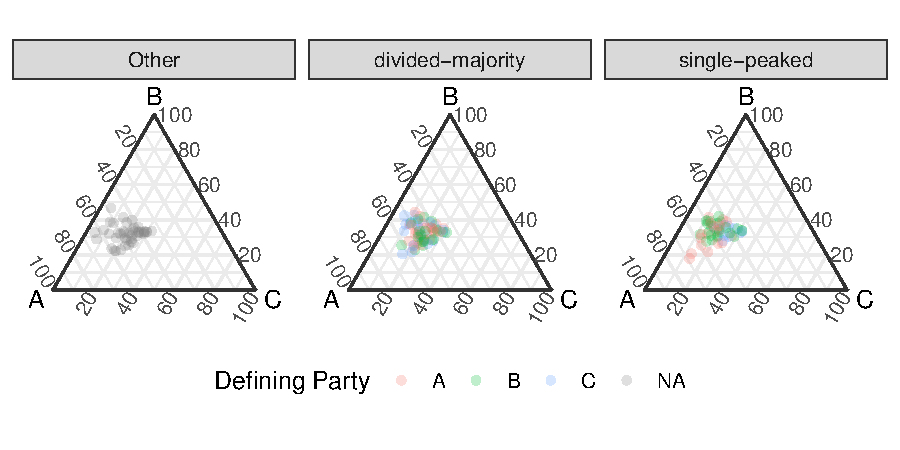
\includegraphics[width = \textwidth]{../output/figures/cses_fp.pdf}
	\caption{Distribution of first preferences in CSES cases, by class}
	\label{fig:cses_fp}
\end{figure}

The CSES dataset comprises a total of 162 cases, with a mean of 1384 and a standard deviation of 539 respondents per case.\footnote{Minimum: 360 respondents, Hong Kong 2004; maximum: 3795, New Zealand 1996.} Of these, we discarded two (Belarus 2008 and Lithuania 1997), because no respondent has complete preferences over all three parties. Within each case, we applied the label $A$ to the party that most respondents stated as first preference; the label $B$ to the party that the second-most respondents stated as second preference; and, finally, the label $C$ to the party that the third-most respondents stated as their first preference. Thus, the expected ballot profile for all of the cases is $v_A > v_B > v_C$. 

Figure~\ref{fig:cses_fp} plots the distribution of first preferences for each case on a ternary diagram. Given the above labelling convention, the distribution is tightly packed into one part of the simplex, its boundaries delineated by the $(1 - v_C) / 2$ boundary on the one side, and the $(1 - v_B) / 2$ on the other.\footnote{Conceptually, this makes sense: a violation of the first one would suggest that $v_B > v_A$, and a violation of the second one would suggest that $v_C > v_B$.} The figure groups together cases that share characteristics in second preferences (single-peaked, i.e. defining party is attractor; divided majority, i.e. defining party is repeller; and all others). There is no discernible difference in the distribution of first preferences between the groups, and there is no discernible difference in the distribution conditional on the defining party. Note that even though the distribution is strongly centred on a particular part of the simplex, our labelling convention is WLOG: the results remain representative.

\vspace*{2em}
\begin{center}
[\textbf{GIS plot with countries contained in CSES data} here]
\end{center}
\vspace*{2em}

Next, we point out an empirical regularity across the CSES cases: they tend to conform relatively well to the single-peaked -- neutral -- divided majority spectrum. (Point out any potential outliers)

\vspace*{2em}
\begin{center}
[\textbf{Visualisation of second preference distribution in CSES data} here]
\end{center}
\vspace*{2em}

\subsection{Methods}

\todo[inline]{(So far, so good. We have described the data and justified the CSES.) Separate description of "methods" necessary?}

After calculating the strategic incentive for each voter in each case, and at different levels of $s$, we can perform further analyses to examine the three questions set out in the introduction of this section. First, we hold $s = 85$ constant and check to what extent strategic incentives by \emph{voter type} conform to the predictions made in the theoretical section. We do this by comparing conditional probabilities of strategic votes $YXZ$ and $ZXY$ being optimal for a $XYZ$ voter in each case in the CSES. Formally, we look at the distributions $\Prob(YXZ | XYZ \land C)$ and $\Prob(ZXY | XYZ \land C)$ where $C$ is one of the previously defined second-preference distribution classes ($A+$, $B+$, $\ldots$)

For comparing the extent and magnitude of incentives overall, we aggregate the proportions across both voter types and cases. Here, we are interested in the overall proportion of positive strategic incentives at different levels of information under both plurality and RCV. Furthermore, we also compare the proportion of voters with $\tau > 0$ under both RCV and plurality in each case, respectively. (\emph{What about interdependence?})

Finally, we perform analyses of overall performance of the two electoral systems. For each case, we calculate the probability of different voting paradoxes (non-monotonicity [RCV], no-show [RCV], [plurality]) to check which of the electoral systems is more vulnerable, given the empirical distribution of ballot profiles. We also check which of the two electoral systems is more likely to benefit the Condorcet winner, and how much of a difference strategic voting makes in terms of changing the winner (how?)

\section{Results: Strategic Voting by Second Preference Class}

To be included. Boxplots, scatterplots, etc. See \texttt{checking\_cases.pdf}.

\section{Results: Incentives}

\begin{figure}[!h]
	\centering
	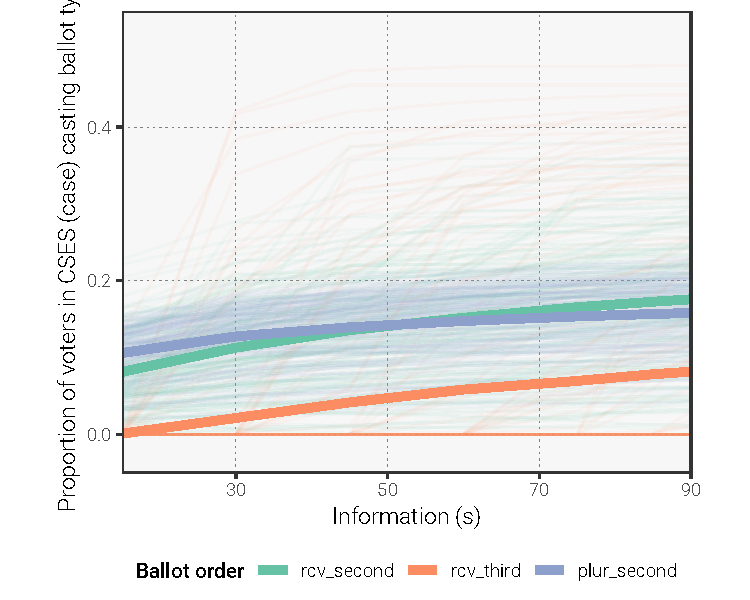
\includegraphics[width = .6 \textwidth]{../output/figures/cses_freq.pdf}
	\caption{Proportion of voters with non-sincere optimal vote, by level of information. Left panel: NSW. Right panel: CSES}
	\label{fig:sv_prop}
\end{figure}

What can we see here? The plot describes the proportion of voters in each case that, conditional on the level of information, $s$, have a strategic incentive to either rank their second preference first (RCV second) or their third preference first (RCV third), and to vote for their second preference under plurality (Plurality second).
The aggregate pattern is extremely similar across both cases. At very low levels of information, there are roughly similar proportions of RCV second and plurality second optimal votes (with plurality being slightly higher). There exists virtually no incentive to vote RCV third. This changes as information improves: the plurality incentive stagnates below 0.2 on average, whereas RCV second keeps rising. Crucially, at high levels of information, the incentive to vote RCV third also becomes very large. (how is this related to the theory?)

The hypothesised reason for this is that in very low information environments, the "strong pushover" (i.e., putting your third preference first on the RCV ballot) may accidentally elect one's third preference. With more precise beliefs, this is unlikely to occur.

\textit{Main takeaways:}
\begin{itemize}
\item Overall proportion of strategic voters in high-information environments is higher under RCV than it is under plurality (but this doesn't say anything yet about the magnitude of these incentives!)
\item "Strong pushover" only occurs at very high levels of information.
\end{itemize}

\subsection{Direct Comparison of Frequency}

\begin{figure}[!h]
	\centering
	\includegraphics[width = .6 \textwidth]{"../output/figures/cses_prop"}
	\caption{Proportion of voters with non-sincere optimal vote, by level of information. Left panel: NSW. Right panel: CSES}
	\label{fig:sv_dist}
\end{figure}

Figure~\ref{fig:sv_dist} plots the proportion of "optimal" strategic voters under RCV and Plurality for each case seperately. This further supports the conclusions from the previous section: For the most part, the proportion of strategic voters under plurality remains capped at around $\approx 0.2$. For low levels of $s$, the cases are distributed around very low levels of strategic voting under both electoral systems. However, as information increases, the proportion of voters with a positive incentive under AV increases dramatically.

What explains the odd pattern in the Australian case? Most cases seem to scatter pretty clearly around a proportion of $\approx 0.18$ for plurality. This is a consequence of using the same set of ``voters'' every time: the proportion of Green voters remains fixed; and in most cases in NSW, Greens face a \textit{very} strong incentive to abandon their first preference under plurality. The few outliers to the right of the $0.18$ plurality value are those cases where the Greens are strong enough such that supporters of other parties have an incentive of abandoning those instead. 

Given that an information environment of $s \approx 85$ is feasible (Eggers and Vivyan, 2018), it would seem as if strategic voting under RCV is not just feasible, but should also concern a strong minority of voters. Why, then, is this not something that political debates about RCV have picked up so far? (1) So far, we don't know how large that incentive to vote strategically is. It may be extremely small, and, assuming costs to strategic voting, ultimately not worth it. (2) Parties may have incorporated such strategic considerations in their how-to-vote cards, thus reducing costs for voters. (Can we check this empirically?)

\subsection{QQ-Plots}

\begin{figure}[!h]
	\centering
	\includegraphics[width = .6 \textwidth]{"../output/figures/cses_qq"}
	\caption{QQ-Plot of strategic incentives, $\tau$, under Plurality (x) and RCV (y). Left panel: NSW. Right panel: CSES.}
	\label{fig:qqplots}
\end{figure}

So we see that under RCV, incentives to vote strategically exist. But exactly how large are these incentives: do they warrant acting upon? Fortunately, our approach of calculating pivotal probabilities and expected utilities allows us to quantify the exact strategic incentive ($\tau$, see also Eggers and Vivyan 2018). 

Figure~\ref{fig:qqplots} compares the distribution of strategic incentives under both plurality and RCV, conditional on $s$, in QQ-Plots. A couple of general observations: (1) The greater $s$, the greater the variance in both $\tau_{RCV}$ and  $\tau_{P}$. This makes sense: when I know very little about the likely electoral outcome, voting sincerely is a less risky strategy, and incentives to vote strategically are smaller. (2) For any level of $s$, \textit{negative} strategic incentives (i.e., situations where the sincere vote is the optimal vote) are relatively more common. (3) Conversely, for any level of $s$, (small and moderate) \textit{positive} strategic incentives are more common under plurality. This is not true of very high levels of $\tau$, which are, again, more common under RCV (see how the aggregate line crosses the 45-degree line in the CSES panel again). (4) The Australian case features smaller incentives to vote strategically overall (?) -- this may have to do with the relative weakness of the Greens. 

The main takeaway here is that strategic voting under RCV, for the most part, brings smaller benefits compared to a sincere vote. There are, however, a few situations at the extreme end where there is a very high incentive under RCV.

What this means is that if we assume strategic voting to be costly (relative to a sincere vote), then we would observe much less of it in RCV. This is equivalent to calculating $\hat{\tau} \equiv \tau - c$, where $c$ is a constant cost. Under RCV, this would shift a much greater part of the distribution into the negative domain, thus attenuating any strategic incentive.

\section{Results: Electoral System Performance}
\subsection{Incidence of Voting Paradoxes}

\begin{figure}[!h]
	\centering
	\includegraphics[width = .6 \textwidth]{"../output/figures/paradoxes_cses"}
	\caption{Probability of voting paradoxes under RCV over probability of wasted vote under plurality. Left panel: NSW. Right panel: CSES}
	\label{fig:paradox}
\end{figure}

Figure~\ref{fig:paradox} plots the probability of different voting paradoxes under RCV over the probability of wasting one's vote under plurality. This is conditional on $s = 85$. In both cases, there is a higher chance of the non-monotonicity paradox occuring than there is of the the no-show paradox occuring. However, in either situation this is overshadowed by the much higher probablity of casting a wasted vote under plurality: the entire sample fits to the right of the 45-degree line. What this suggests is that, no matter what the strategic voting incentives, RCV is much better at avoiding tricky electoral situations.

\textit{(Need to check why in the Australian case Pr(Wasted Vote) begins at $\approx 0.2$)}

Also note that the LOESS in the Australian case probably suffers from overfitting - one or two observations towards the high end of Pr(Wasted Vote) pull the non-mon curve downwards.

\subsection{Interdependence} \label{interdep}

\begin{figure}[!h]
	\centering
	\includegraphics[width = .6 \textwidth]{"../output/figures/cses_l0"}
	\caption{Proportion of voters whose Level-2 strategic vote differs from their sincere vote, conditional on proportion of Level 2 strategic voters in population ($\lambda$). Left panel: NSW. Right panel: CSES.}
	\label{fig:figure1}
\end{figure}

\begin{figure}[!h]
	\centering
	\includegraphics[width = .6 \textwidth]{"../output/figures/cses_l1"}
	\caption{Proportion of voters whose Level-2 strategic vote differs from their Level-1 strategic vote, conditional on proportion of Level 2 strategic voters in population ($\lambda$). Left panel: NSW. Right panel: CSES.}
	\label{fig:figure1}
\end{figure}

Need to provide interpretation still.

\subsection{Condorcet Winner}

\section{Conclusion}

\end{document}